\documentclass[10pt,letterpaper,onecolumn,draftclsnofoot]{IEEEtran}
\usepackage[margin=0.75in]{geometry}
\usepackage{listings}
\usepackage{color}
\usepackage{longtable}
\usepackage{graphicx}
\usepackage{float}
\usepackage{tabu}
\definecolor{dkgreen}{rgb}{0,0.6,0}
\definecolor{gray}{rgb}{0.5,0.5,0.5}
\definecolor{mauve}{rgb}{0.58,0,0.82}

\graphicspath{{../images/}}

\lstset{frame=tb,
language=C,
columns=flexible,
numberstyle=\tiny\color{gray},
keywordstyle=\color{blue},
commentstyle=\color{dkgreen},
stringstyle=\color{mauve},
breaklines=true,
breakatwhitespace=true,
tabsize=4
}

\setlength{\parindent}{0cm}

\begin{document}
\begin{titlepage}
	\title{CS 461 - Fall 2016 - Technology Review}
	\author{Matthew Johnson}
	\date{\today}
	\maketitle
	\vspace{4cm}
	\begin{abstract}
		\noindent Abstract goes here
	\end{abstract}

\end{titlepage}
\tableofcontents
\clearpage

\section{Programming Languages}

At the highest level, a main component of our software defined network
implementation is the programming language it is written in. This is an
important decision to make early in our design, as it affects all choices that
follow.

\subsection{Options}

\subsubsection{Go}

Our first choice is the Go programming language. This is naturally the strongest
choice as the rest of the Ciao infrastructure is written in Go. It would require
a very strong argument to create a separate networking mode in another language.
While technically possible, it would require a great deal of work to make the
different pieces compatible with each other.

\subsubsection{C}

Other than interaction with the rest of the Ciao project, C is another natural
choice. C has been around for decades, and has the capability to do nearly every
computational and networking task. The libraries are extensive and available and
the language is fast.

\subsubsection{Python}

Python is a choice here simply because of its ease of use. Python is very
expressive and has nice libraries that abstract away the complicated details of
software defined networking. The main downfalls of Python, however, are its
reduced speed and space efficiency compared to Go and C. A result of writing a
cloud orchestrator in Python is exemplified in the extremely complicated and
slow Openstack project~\cite{uglyopenstack}.

\subsection{Goals for use in design}

As stated, the choice of programming language will affect all aspects of our
design for this project, from code structure to networking libraries and module
design. This choice will easily have the largest impact on our project.

\subsection{Criteria being evaluated}

Important criteria to consider is the availability of necessary libraries and of
the language and its dependencies itself, the inherent speed of the language to
be used, the security features the language offers, the concurrency
capabilities, and the overall ease of use.

\subsubsection{Availability}

The most available language in terms of libraries and the language itself
(regarding its standard libraries) is obviously C because of how ubiquitous it
is, how universally available it is, and how extensive its standard libraries
are~\cite{SOC}.

Close behind C in availability is Python. Python is nearly as available as C is
because of how popular it has become in the last ten years~\cite{PYPL}. Python
has many libraries that provide simple abstractions to networking
functionalities.

Of all these languages, Go is the least available as it is the youngest and
least popular of the three. Go is not normally available by default on most
operating systems and must be installed by the user. Go does, however, have
available libraries that make it very easy to implement networking, as is
evidenced by the extent to which they are used in the Ciao project
currently~\cite{ciao}.

The following figure demonstrates the popularity of C, Go, and Python in the
United States in the last ten years.

\begin{figure}[H]
	\begin{center}
		\makebox[\textwidth]{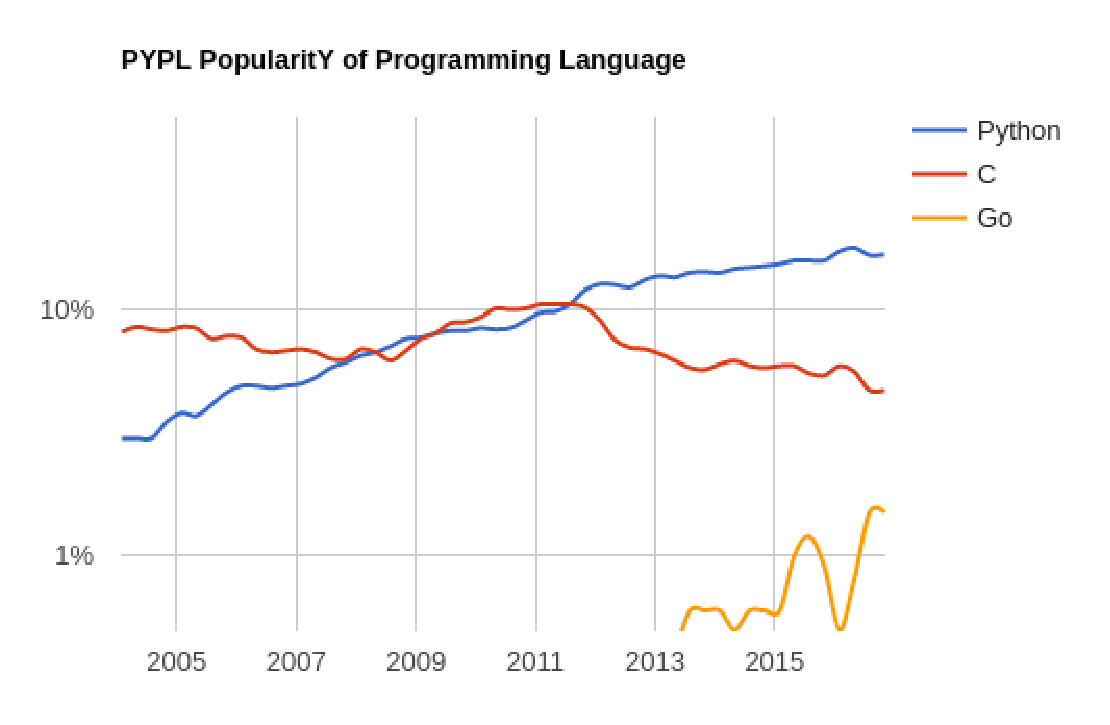
\includegraphics[width=10cm]{pythoncgo.eps}}
		\caption{Python, C, and Go popularity in the US~\cite{PYPL}}
	\end{center}
\end{figure}

\subsubsection{Speed and Space Efficiency}

One benefit of lower-level languages like Go and C is how they treat their
variables. Go and C treat variables differently than some languages such as
Python, which create overhead in order to track type information, and Java,
which converts small ints to Integer class instances when placing them in a
list. An example of this is in the representations of the same value in Go,
Python, and C~\cite{davecheney}:

\begin{lstlisting}
var gocon int32 = 2014              // Go:      4 bytes
uint32_t gocon = 2014;              // C:       4 bytes
gocon = 2014                        #  Python: 24 bytes
\end{lstlisting}

Go performs comparably to C with regard to speed, as well~\cite{benchmarks},
which is considerable since C is often the standard for fast programming
languages. Compared to Python, as would be expected, Go and C can perform up to
45 times faster depending on the workload~\cite{benchmarks}.

\subsubsection{Concurrency}

Concurrency is a key consideration for programming languages when implementing a
software defined network. All operations must happen quickly and in parallel and
must scale effortlessly. Therefore, it is necessary that all operations run in
their own individual threads.

C has an extensive and established framework for parallel computing by utilizing
pthreads. Mutexes can help the programmer protect against race conditions in
their code, but the responsibility is up to the programmer to make their
software thread-safe.

Python has similar tools as C, but the parallelization is handled by a global
interpreter lock (GIL). The GIL is a "mutex that prevents multiple native
threads from executing Python bytecodes at once." GIL is necessary in python
because the underlying C code that implements python is not thread-safe. The GIL
"prevents multithreaded CPython programs from taking full advantage of
multiprocessor systems in certain situations"~\cite{GIL}.

Go, on the other hand, combines the power of C and the ease of use and
lock-handling of Python. You can use goroutines (functions that are capable of
running concurrently with other functions) to create concurrency. Utilization of
goroutines and other builtin language functionalities make concurrency very easy
and lightweight in Go. An example from golang-book.com demonstrates how simple
and lightweight threads in Go can actually be~\cite{goroutines}:

\begin{lstlisting}
package main

import "fmt"

func f(n int) {
	for i := 0; i < 10; i++ {
		fmt.Println(n, ":", i)
	}
}

func main() {
	go f(0)
	var input string
	fmt.Scanln(&input)
}
\end{lstlisting}

\subsubsection{Ease of use}

Python is by far the easiest to learn, use, and read. It focuses on
"readability, coherence, and software quality" and is recognized by many to be
extremely easy to use~\cite{learningpython}

C, being the oldest and lowest-level language of the three, is not a simple
language to work with. Many things that are normally abstracted away in other
languages are required to be programmed explicitly by the programmer. String
manipulation is especially difficult in C.

Go is easier to learn than C and makes many improvements in terms of ease of
use. It was even designed this way. Go was designed to make programming
efficient in large-scale software development across teams with varying levels
of experience and skill. It was designed with "built-in concurrency and garbage
collection" and includes "rigorous dependency management."~\cite{godesign}.
These features are important for the work required by this project.

Another important note is that the rest of Ciao is written in Go, and while
possible to create interfaces from C or Python for Go, it would be very
difficult. Another option would be to re-implement Ciao in another language,
which is so difficult and time consuming that it cannot even be considered as an
option. With this consideration, Go is the clear winner in terms of ease of use.

\subsection{Direct Comparison}

\begin{center}
	\begin{tabular}{| l | l | l | l | l | l |}
		\hline
		Language & Availability & Efficiency & Concurrency & Ease of use
		\\ \hline
		Go     & 3 & 1 & 1 & 1 \\ \hline
		C      & 1 & 2 & 2 & 3 \\ \hline
		Python & 2 & 3 & 3 & 2 \\ \hline
	\end{tabular}
\end{center}

\subsection{Selection}

Based on the criteria explored above, the Go programming language is the
language we are selecting to implement our solution in. The remainder of the
technical review will be based on the assumption that we will be implementing
our solution in Go.

\section{Networking Libraries}

\subsection{Options}

\subsubsection{}

\subsubsection{}

\subsubsection{}

\subsection{Goals for use in design}

\subsection{Criteria being evaluated}

\subsubsection{Availability}

\subsubsection{Speed}

\subsubsection{Security}

\subsubsection{Concurrency}

\subsection{Discussion}

\subsection{Selection}

\section{Functional Testing Frameworks}

\subsection{Options}

\subsubsection{}

\subsubsection{}

\subsubsection{}

\subsection{Goals for use in design}

\subsection{Criteria being evaluated}

\subsubsection{Availability}

\subsubsection{Speed}

\subsubsection{Security}

\subsubsection{Concurrency}

\subsection{Discussion}

\subsection{Selection}

% Cody
\section{Packet Level Protocols}
One of the main components of our system is deciding which protocol will be
used to move data from one node to the next. Ciao provides its own data
transfer protocol using SSNTP. Comparing how SSNTP works in general to other
data transfer formats will provide insight into which protocol should be used.

\subsection{Options}

\subsubsection{SSNTP}
Simple and Secure Node Transfer Protocol is Intel's solution for the transfer
of data inside of Ciao networks. It is based on Transport Layer Security (TLS),
the defacto standard for secure data transfer over the Internet. Part of what
sets Ciao apart from the competition is its simplicity, as well as concise
message format.\cite{ssntp}

\subsubsection{TLS}
Transport Layer Security, or TLS, is the contemporary standard for secure data
transfer across the Internet. It was built as an improvement upon the Secure
Socket Layer protocol. It has great appeal as it is widely utilized, modern,
and well studied.\cite{tls}

\subsubsection{SSL}
Secure Socket Layer, or SSL, was the first version of what eventually became
TLS following its third major revision. Originally utilized in Netscape, it
wasn't widely utilized until it's third major revision. Secure Socket Layer
encrypts at the application layer, allowing broad general use. While being
somewhat older than the other protocols on the list, it is well understood and
the security has been well proven.\cite{ssl}

\subsection{Goals for use in design}
The primary goal of the selected protocol is fast, stable, secure, and
scalable communication between compute nodes and the orchestration node in
Ciao. These are simple, but critical goals for the project.

\subsection{Criteria being evaluated}
The criteria for each protocol will be their security capabilities, protocol
overhead, and ease of use. While stability is a concern, each protocol has
shown stability through implementation in other applications many times over.
This will be less of a focus for evaluation purposes.

\subsubsection{Speed}
Speed is a major consideration when working with a software defined network.
Our final selection for a protocol needs to be fast. Any major delays in 
communication due to encryption or protocol overhead is a concern. While each
implementation of the protocol will have its pros and cons, here the focus
will be on application overhead to keep the metric in measurable territory.

SSL has two major components, the protocol, and the handshake protocol. The
handshake protocol is important as it ensures the overall security and
authenticity of the communication between point A and point B. 

%Diagram of SSL handshake here
\begin{figure}[H]
	\begin{center}
		\makebox[\textwidth]{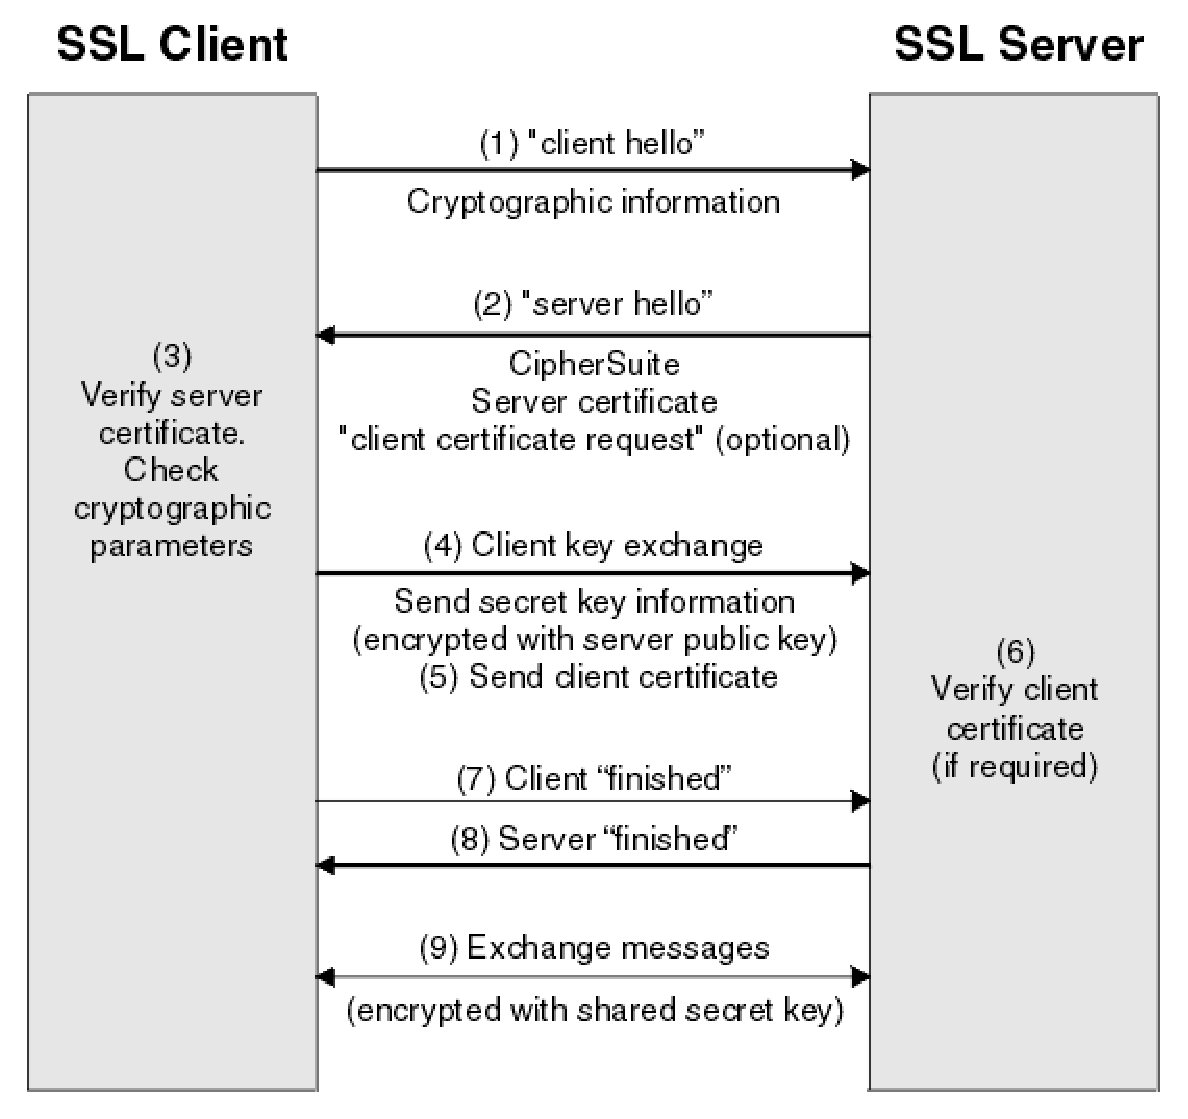
\includegraphics[scale=.35]{ssl-diag.eps}}
		\caption{Simple SSL and TLS Handshake\cite{ibm-diagram}}
	\end{center}
\end{figure}

The SSL/TLS handshakes are identical, but 



\cite{topdown-ssl}

\subsubsection{Security}

\subsubsection{Accessibility}

\subsection{Discussion}

\subsection{Selection}

%----------------------

\section{nvGRE and VxLAN Switches}

\subsection{Options}

\subsubsection{nvGRE}

\subsubsection{VxLAN}

\subsubsection{}

\subsection{Goals for use in design}

\subsection{Criteria being evaluated}

\subsubsection{Availability}

\subsubsection{Speed}

\subsubsection{Security}

\subsubsection{Concurrency}

\subsection{Discussion}


\subsection{Selection}

%----------------------

\section{GRE/Linux Bridges}

\subsection{Options}

\subsubsection{Linux Bridges}

\subsubsection{}

\subsubsection{}

\subsection{Goals for use in design}

\subsection{Criteria being evaluated}

\subsubsection{Availability}

\subsubsection{Speed}

\subsubsection{Security}

\subsubsection{Concurrency}

\subsection{Discussion}

\subsection{Selection}


%End Cody

\section{References}

\bibliographystyle{IEEEtran}
\bibliography{tech}

\end{document}
